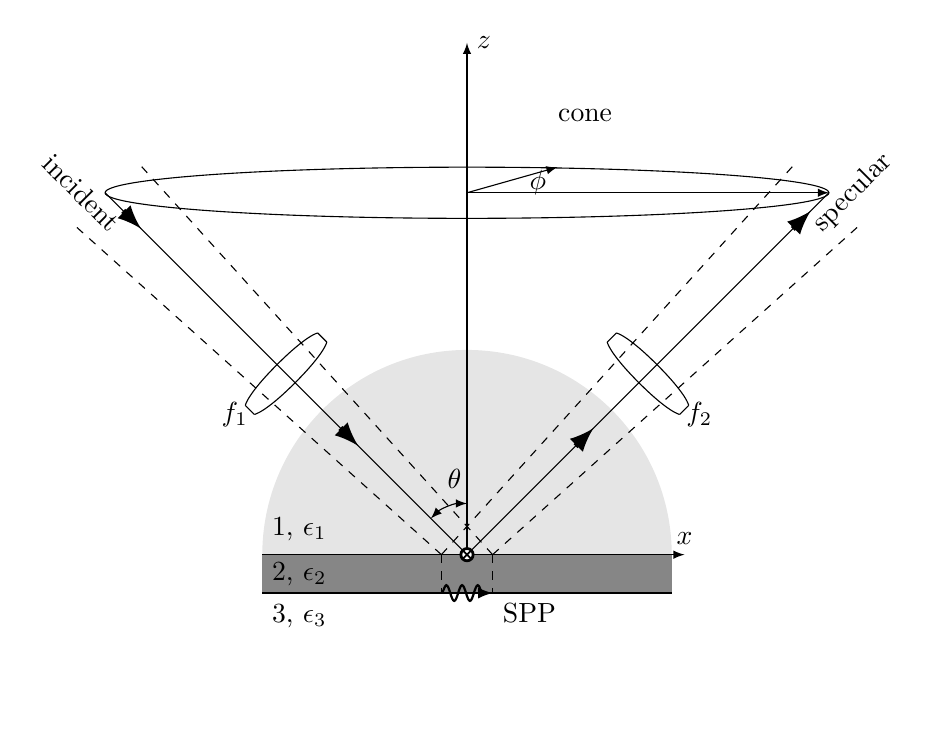
\begin{tikzpicture}[
    scale=0.65,
    >=latex,
    media/.style={font={}},
    wave/.style={%
        decorate,decoration={snake,post length=1.0mm,amplitude=1mm,
        segment length=2.0mm},thick},
    interface/.style={%
        % The border decoration is a path replacing decorator.
        % For the interface style we want to draw the original path.
        % The postaction option is therefore used to ensure that the
        % border decoration is drawn *after* the original path.
        postaction={draw,decorate,decoration={border,angle=-45,
                    amplitude=0.3cm,segment length=2mm}}},
    ]

    \def\thetasp{45}
    \def\spread{10}
    \def\wx{1}
    \def\conedist{10}

    % glass
    \fill[gray!20] (4,0) arc (0:180:4);

    % air
    \fill[gray!0] (-4,-3) rectangle (4,0);

    % metal
    \fill[gray!95] (-4,-0.75) rectangle (4,0);

    % Interface
    \draw[black,line width=.5pt](-4,0)--(4,0);
    \draw[black,line width=.5pt](-4,-0.75)--(4,-0.75);

    % Vertical dashed line
    %\draw[dashed,gray](0,-3)--(0,3);
    % Coordinates system
    \draw[<->] (4.25,0) node[above]{$x$}-|(0,10) node[right]{$z$};
    \draw[->] (0,{cos(\thetasp)*\conedist}) -- ({sin(\thetasp)*\conedist}, {cos(\thetasp)*\conedist});
    \draw[->] (0,{cos(\thetasp)*\conedist}) --
    ({0.25*cos(\thetasp)*\conedist}, {0.5+sin(\thetasp)*\conedist})
    node[shift={(-0.25,-0.20)}] {$\phi$} ;

    \node[shift={(1.5,{sin(\thetasp)*\conedist-1.5})}] {cone};

    % cone
    \draw (0,{cos(\thetasp)*\conedist}) ellipse ({sin(\thetasp)*\conedist} and 0.5);

    % Incidence
    %\draw[->,wave]
    %     (135:3.2cm)--(135:2.5cm)node[right]{$E_0$};
    \draw[dashed](0:{\wx*-0.5})--({90+\thetasp+\spread*0.5}:10);
    \draw[](0:0)--({90+\thetasp}:10) node[rotate={270+\thetasp}, shift={({0.30*cos(270-\thetasp)},{0.30*sin(270-\thetasp})}] {incident};
    \draw[<->] (0,1) arc (90:{90+\thetasp}:1) node[shift={(0.3,0.5)}] {$\theta$};
    \draw[->,line width=2pt]({90+\thetasp}:9.5)--({90+\thetasp}:9.0);
    \draw[->,line width=2pt]({90+\thetasp}:3.5)--({90+\thetasp}:3.0);
    \draw[dashed](0:{\wx*0.5})--({90+\thetasp-\spread*0.5}:10);
    %\draw[->](0,0.75)arc(90:135:.75cm);

    % Reflection
    %\draw[->,wave]
    %     (45:2.5cm)--(45:3.2cm)node[right]{$E_r$};
    \draw[dashed](0:{\wx*-0.5})--({90-\thetasp+\spread*0.5}:10);
    \draw[](0:0)--({90-\thetasp}:10) node[rotate={90-\thetasp},
    shift={({0.30*cos(270+\thetasp)},{0.30*sin(270+\thetasp})}] {specular};
    \draw[<-,line width=2pt]({90-\thetasp}:9.5)--({90-\thetasp}:9.0);
    \draw[<-,line width=2pt]({90-\thetasp}:3.5)--({90-\thetasp}:3.0);
    \draw[dashed](0:{\wx*0.5})--({90-\thetasp-\spread*0.5}:10);
    \draw[dashed]({\wx*0.5},0)--({\wx*0.5},-0.75);
    \draw[dashed]({-\wx*0.5},0)--({-\wx*0.5},-0.75);
    \draw[->,wave,color=black]
     ({-\wx*0.5},-0.75)--({\wx*0.5},-0.75) node[right,shift={(0,-0.25)}]{SPP};


    % first lens
    \def\lenswidth{2}
    \def\lensheight{0.25}
    \def\lensbow{0.125}
    \def\lensshift{({-5*sin(\thetasp)},{5*cos(\thetasp)})}
    \def\lensrotate{\thetasp}
    \draw[shift={\lensshift}, rotate={\lensrotate}]({-\lenswidth/2},{-\lensheight/2})--({-\lenswidth/2},{\lensheight/2});
    \draw[shift={\lensshift}, rotate={\lensrotate}]({\lenswidth/2},{-\lensheight/2})--({\lenswidth/2},{\lensheight/2});

    \draw[shift={\lensshift}, rotate={\lensrotate}] plot [smooth, tension=1.5] coordinates {%
    ({\lenswidth/2},{-\lensheight/2})
    (0,{-\lensheight/2-\lensbow})
    ({-\lenswidth/2},{-\lensheight/2})
    } node[shift={(-0.25,0)}] {$f_1$};

    \draw[shift={\lensshift},rotate={\lensrotate}] plot [smooth, tension=1.5] coordinates {%
    ({-\lenswidth/2},{\lensheight/2})
    (0,{\lensheight/2+\lensbow})
    ({\lenswidth/2},{\lensheight/2}) };

    % second lens
    \def\lensshift{({5*sin(\thetasp)},{5*cos(\thetasp)})}
    \def\lensrotate{-\thetasp}
    \draw[shift={\lensshift}, rotate={\lensrotate}]({-\lenswidth/2},{-\lensheight/2})--({-\lenswidth/2},{\lensheight/2});
    \draw[shift={\lensshift}, rotate={\lensrotate}]({\lenswidth/2},{-\lensheight/2})--({\lenswidth/2},{\lensheight/2});

    \draw[shift={\lensshift}, rotate={\lensrotate}] plot [smooth, tension=1.5] coordinates {%
    ({-\lenswidth/2},{-\lensheight/2})
    (0,{-\lensheight/2-\lensbow})
    ({\lenswidth/2},{-\lensheight/2})
    } node[shift={(0.25,0)}] {$f_2$};

    \draw[shift={\lensshift},rotate={\lensrotate}] plot [smooth, tension=1.5] coordinates {%
    ({-\lenswidth/2},{\lensheight/2})
    (0,{\lensheight/2+\lensbow})
    ({\lenswidth/2},{\lensheight/2}) };


   % Media names
    \path[media] (-4,.5)  node[anchor=west] {1, $\epsilon_1$}
                 (-4,-.375) node[anchor=west] {2, $\epsilon_2$}
                 (-4,-1.2) node[anchor=west] {3, $\epsilon_3$};

    % $x$ axis
    \filldraw[fill=white,line width=1pt](0,0)circle(.12cm);
    \draw[line width=.6pt] (0,0)
                          +(-135:.12cm) -- +(45:.12cm)
                          +(-45:.12cm) -- +(135:.12cm);
    % To-paths are really useful for drawing curved lines. The above
    % to path is equal to:
    %
    % \draw[-latex,thick](3.2,0.5)node[right]{$\mathsf{S_{1,2}}$}
    %      ..controls +(180:.2cm) and +(up:0.25cm) .. (3,0);
    % Internally the to path is translated to a similar bezier curve,
    % but the to path syntax hides the complexity from the user.

    % SPP
    %\draw[->,wave,color=black]
    %     (-2,-1.75)--(2,-1.75) node[right]{SPP};

\end{tikzpicture}
